\documentclass[11pt,a4paper]{article}
\usepackage[utf8]{inputenc}
\usepackage[margin=0.8in]{geometry}
\usepackage{amsmath,amssymb,amsfonts}
\usepackage{graphicx}
\graphicspath{{figures/}}
\usepackage{booktabs}
\usepackage{tabularx}
\usepackage{hyperref}
\usepackage{xcolor}
\usepackage{float}
\usepackage{microtype}
\usepackage{fancyhdr}
\usepackage{caption}
\captionsetup[figure]{font=small,labelfont=bf}

\hypersetup{
    colorlinks=true,
    linkcolor=blue!70!black,
    citecolor=blue!70!black,
    urlcolor=blue!70!black
}

\setlength{\headheight}{14pt}
\addtolength{\topmargin}{-2pt}

\pagestyle{fancy}
\fancyhf{}
\rhead{ASM-II: Nuclear Explosion vs. Earthquake Discrimination}
\cfoot{\thepage}

\title{\textbf{\Large Discrimination of Underground Nuclear Explosions from Natural Earthquakes Using Seismic Waveforms, Source Physics, and Regularized Machine Learning}\\[0.5em]
\large Advanced Statistical Methods II Course Project Report}

\author{
    \textbf{Rajveer Vora} (ISI Kolkata) \\
    \textbf{Smarak Patel} (ISI Delhi) \\
    \textbf{Tanish Ghosh} (ISI Bangalore) \\[0.5em]
    \href{https://github.com/RajveerVoraUni/nuclear-testing}{GitHub Repository}
}
\date{October -- November 2026}

\begin{document}

\maketitle

\begin{abstract}
Distinguishing underground nuclear explosions from natural earthquakes is an important challenge in global seismic monitoring and nuclear non-proliferation verification under the Comprehensive Nuclear-Test-Ban Treaty. This Advanced Statistical Methods II project develops an integrated signal-processing, statistical learning, and deep learning framework using three-component ($Z, N, E$) seismic waveforms. We extract 18 discriminative features capturing signal energy ratios, spectral characteristics, and three-dimensional polarization, and compare five classical machine learning classifiers: Lasso, Elastic Net, Random Forest, SVM (RBF kernel), and XGBoost. These are evaluated alongside a three-channel 2D CNN trained on $128 \times 128$ time-frequency spectrograms generated using the Short-Time Fourier Transform (STFT). To ensure reliable generalization, model selection and evaluation use five-fold event-grouped cross-validation, with recordings from the same seismic event restricted to a single fold. We also investigate the challenges of extreme class imbalance, demonstrating why ROC-AUC alone may obscure the practical cost of false positives and motivating the use of Precision-Recall AUC (PR-AUC) as a key evaluation metric. The results show strong classification performance across both modeling approaches. Finally, we investigate external generalization using multi-station consensus across six historical North Korean nuclear tests, all withheld from model training and hyperparameter tuning. The framework successfully identifies all six events, providing an additional assessment of its performance beyond the benchmark dataset.
\end{abstract}

\vspace*{0.5em}

\section{Introduction and Problem Formulation}
Underground nuclear detonations generate seismic waves that propagate across continental and teleseismic distances, sharing basic observational similarities with natural tectonic earthquakes. Since the inception of the Comprehensive Nuclear-Test-Ban Treaty (CTBT), the International Monitoring System (IMS) has operated a global network of seismological stations to verify compliance.

From an applied statistical modeling perspective, seismic event discrimination presents three distinct challenges:
\begin{enumerate}
    \item \textbf{High-Dimensional Time-Series \& Non-Stationarity:} Raw seismograms are non-stationary, oscillatory time-series characterized by distinct wave phase packets ($P_n$, $P_g$, $S_n$, $L_g$, and surface waves) arriving across time.
    \item \textbf{Spatial Correlation and Grouping Structure:} A single seismic event is typically recorded by multiple stations globally. A naive random split of station traces produces severe \textit{data leakage}, artificially inflating validation accuracy because the model simply memorizes the event signature rather than learning generalized physics.
    \item \textbf{Severe Class Imbalance in Operational Deployments:} In nature, tens of thousands of earthquakes occur annually, compared to zero or one clandestine nuclear tests. Under such severe imbalance, standard evaluation metrics like Accuracy and ROC-AUC become deceptive, as even a minuscule False Positive Rate generates an overwhelming volume of false alarms.
\end{enumerate}

In this project, we address these challenges through a unified three-component ($Z, N, E$) seismic framework. We examine whether physics-guided feature extraction combined with regularized generalized linear models (Lasso, Elastic Net), modern tree/kernel ensembles (XGBoost, SVM), and end-to-end representation learning (3-Channel 2D CNN) can reliably separate these phenomena.


\section{Historical Motivation}
During the Cold War, the inability to reliably distinguish underground nuclear explosions from natural earthquakes posed a major challenge to international arms-control negotiations. In the absence of dependable verification methods, countries had limited means of independently confirming whether underground nuclear tests were being conducted. Had reliable seismic discrimination techniques been developed earlier, they could have strengthened international monitoring, reduced uncertainty between rival nations, and potentially helped prevent or slow the escalation of the nuclear arms race.

This challenge motivates the use of statistical signal processing. Although explosions and earthquakes both generate seismic waves, their signals can exhibit differences in frequency content, energy distribution, and time-frequency patterns. The Fourier Transform \cite{cooley1965} provides information about a signal's frequency composition, while the Short-Time Fourier Transform (STFT) captures how these frequencies evolve over time through spectrograms.

Building on these techniques, this project investigates whether statistical feature extraction and machine learning can distinguish underground nuclear explosions from natural earthquakes. We compare classical classifiers trained on engineered seismic features with a Convolutional Neural Network trained directly on three-component time-frequency representations.


\section{Physical Foundations and Exploratory Waveform Analysis}
Distinguishing underground nuclear explosions from natural earthquakes relies on fundamental differences in their source mechanics and the resulting seismic wavefield.

\subsection{Source Mechanisms: Isotropic Expansion vs. Shear Slip}
\begin{itemize}
    \item \textbf{Underground Nuclear Explosion:} Modeled as an isotropic pressure pulse radiating outward from an explosive cavity. In the equivalent point-source approximation, the seismic moment tensor is purely diagonal (hydrostatic):
    \begin{equation*}
        \mathbf{M}_{\text{explosion}} = M_0 \mathbf{I}_{3\times3} = \begin{pmatrix} M_0 & 0 & 0 \\ 0 & M_0 & 0 \\ 0 & 0 & M_0 \end{pmatrix}
    \end{equation*}
    Because spherical expansion produces purely radial volume change ($\nabla \times \mathbf{u} \approx 0$), an explosion radiates primary compressional waves ($P$-waves) with virtually no direct shear wave ($S$-wave) excitation at the source.
    
    \item \textbf{Natural Earthquake:} Initiated by frictional shear slip across a planar fault with unit normal $\hat{\mathbf{n}}$ and slip vector $\hat{\mathbf{d}}$ ($\hat{\mathbf{n}} \cdot \hat{\mathbf{d}} = 0$). The resulting double-couple moment tensor is symmetric and traceless:
    \begin{equation*}
        \mathbf{M}_{\text{earthquake}} = M_0 (\hat{\mathbf{n}} \hat{\mathbf{d}}^T + \hat{\mathbf{d}} \hat{\mathbf{n}}^T), \qquad \text{tr}(\mathbf{M}_{\text{earthquake}}) = \sum_{i=1}^3 M_{ii} = 0
    \end{equation*}
    Because shear dislocation involves no net volume change, it directly generates intense transverse shear waves ($S, S_n, L_g$) that oscillate perpendicular to the ray path, depositing substantial energy onto horizontal components ($N, E$).
\end{itemize}

\subsection{Exploratory Analysis: Waveform Structure Comparison}
To empirically investigate these physical differences, Figure~\ref{fig:waveform_comparison} compares synchronized 3-component recordings ($Z, N, E$) of a representative US underground nuclear test (Nevada Test Site, Station MNV) against a moderate natural earthquake (EarthScope GSN, Station TUC). Both events are sampled at 20 Hz, bandpass filtered to $0.8 - 5.0\text{ Hz}$ to isolate body waves from long-period microseisms, and normalized by each event's 3-component peak amplitude ($A_{\text{max}} = \max(|Z|, |N|, |E|)$).

\begin{figure}[htbp]
    \centering
    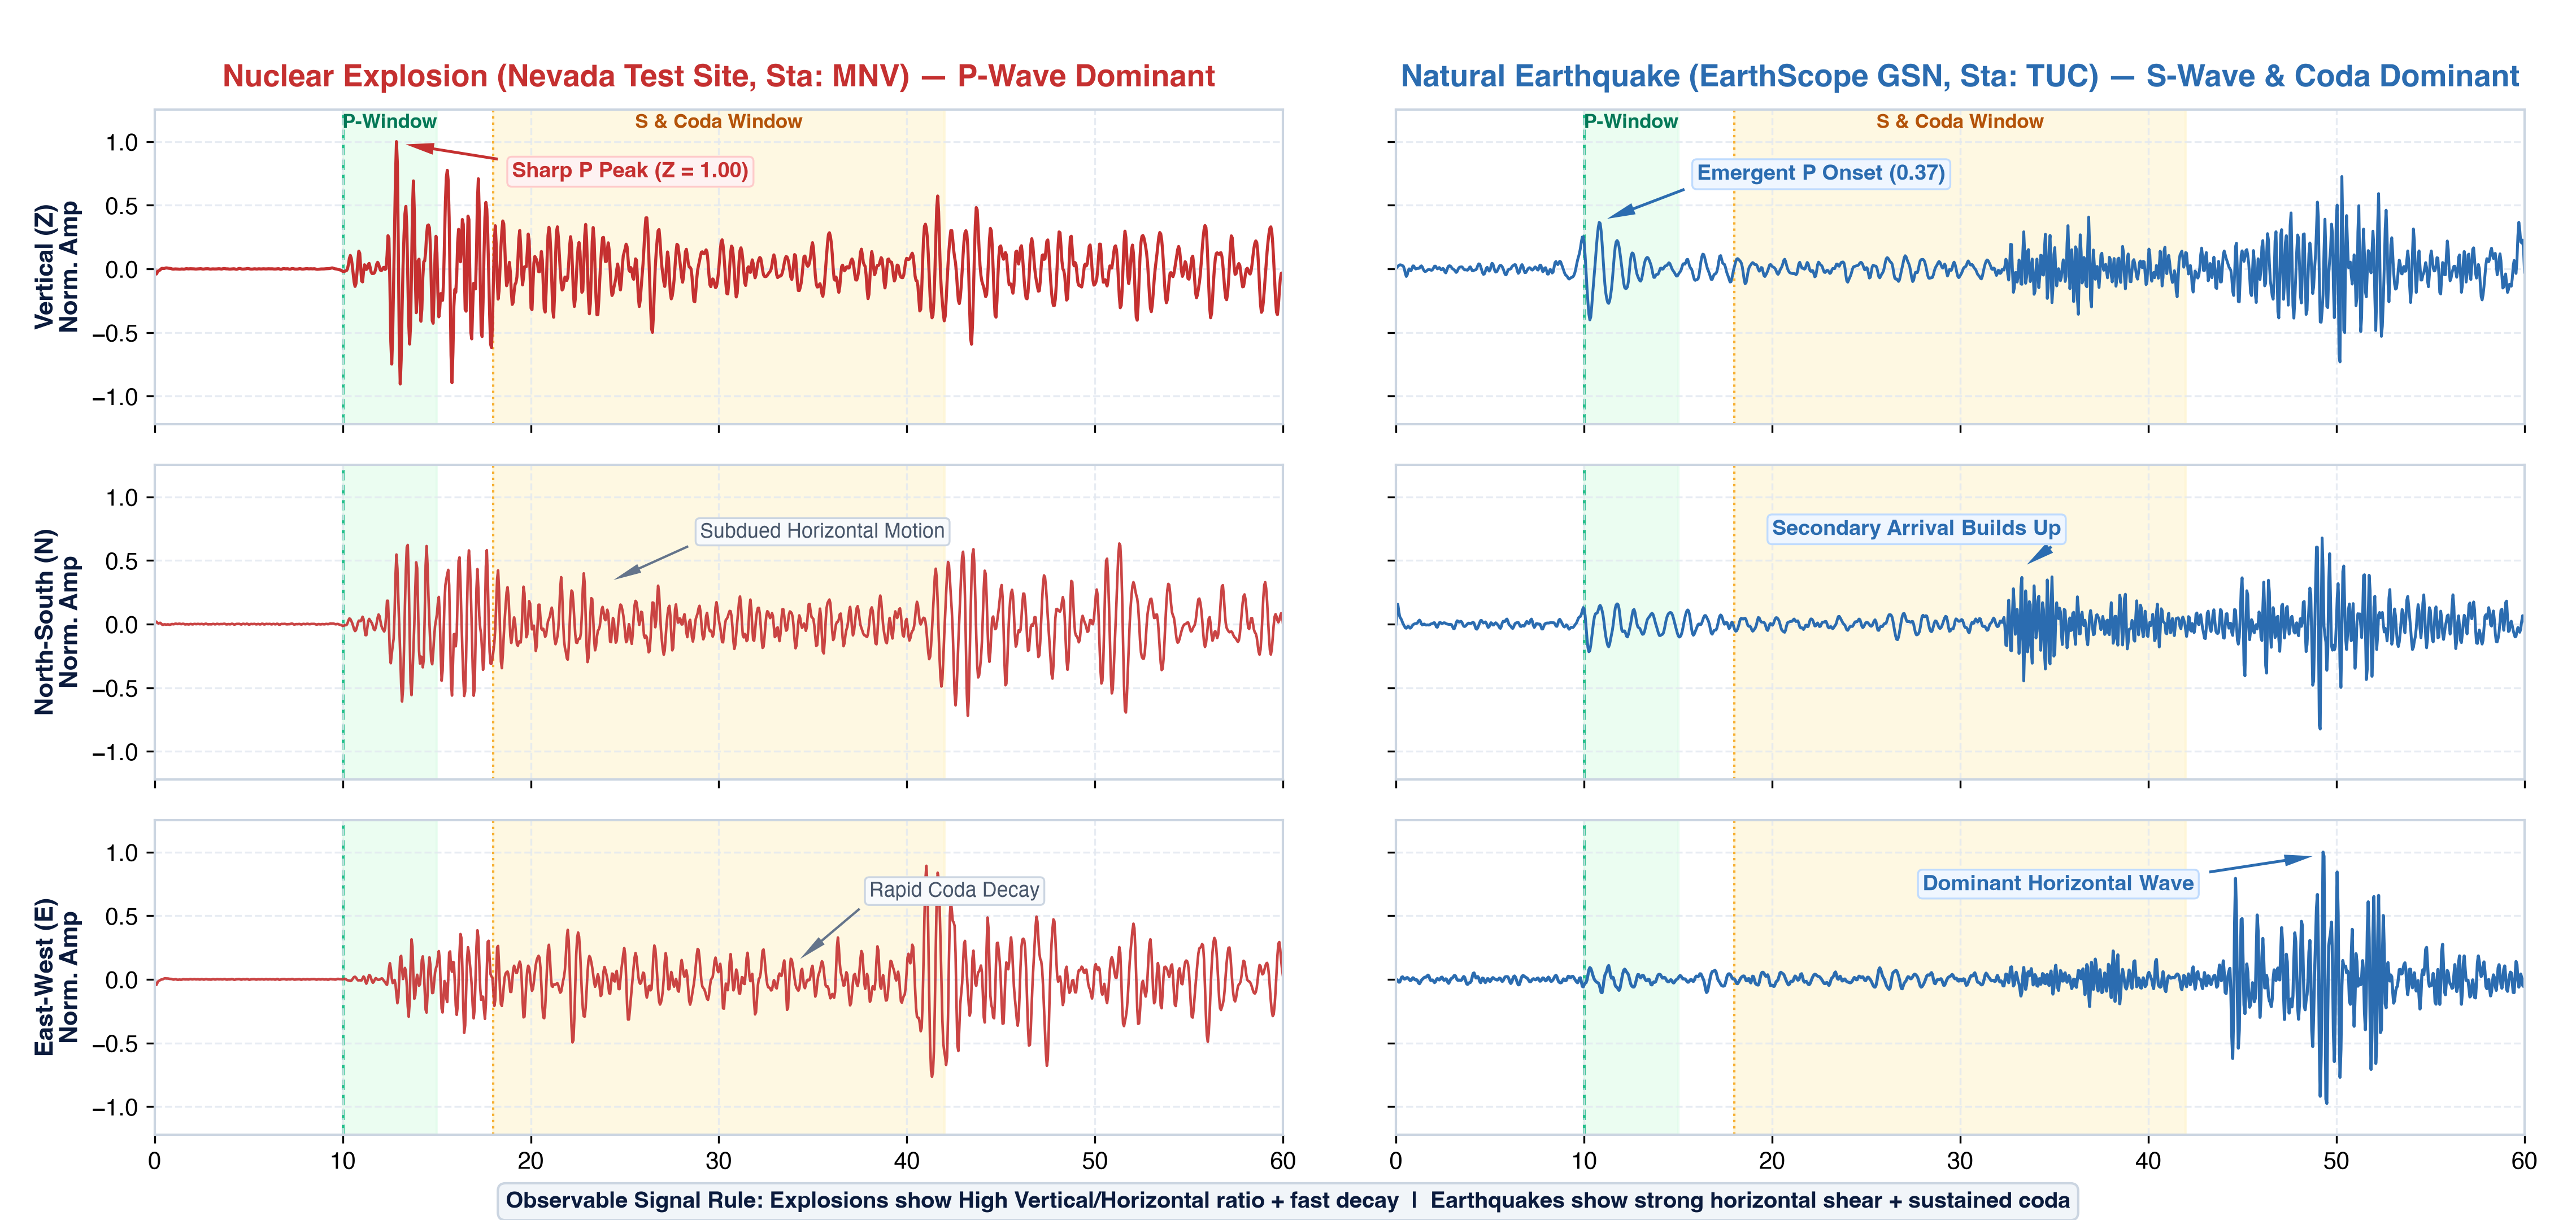
\includegraphics[width=\textwidth]{waveform_comparison.png}
    \caption{\textbf{Exploratory Waveform Comparison between Nuclear Detonations and Natural Earthquakes.} Synchronized 3-component recordings ($Z, N, E$) over a 60-second window. The left column shows a Nevada Test Site underground nuclear explosion (Station MNV); the right column shows a natural tectonic earthquake (Station TUC). Green shaded regions indicate the compressional $P$-wave window ($t \in [10.0, 15.0]\text{ s}$), with $P$-onset aligned at $t_P = 10.0\text{ s}$; amber shaded regions indicate the shear ($S$) and coda window ($t \in [18.0, 42.0]\text{ s}$). Explosions display an impulsive vertical $P$-wave with a severe horizontal shear deficit and rapid decay, whereas earthquakes exhibit an emergent $P$-wave followed by dominant horizontal shear shaking and prolonged coda.}
    \label{fig:waveform_comparison}
\end{figure}

The exploratory comparison reveals three pronounced structural contrasts:
\begin{enumerate}
    \item \textbf{Compressional Dominance vs. Shear Wave Deficit:} In the explosion recording, wave energy is concentrated almost entirely on the vertical component ($Z$) as an impulsive $P$-wave arrival ($A_{\text{norm}} = 1.00$). The horizontal channels ($N, E$) exhibit minimal amplitude ($A_{\text{norm}} < 0.50$), illustrating the classic explosive shear-wave deficit. Conversely, the earthquake's vertical $P$-wave is emergent and moderate ($A_{\text{norm}} \approx 0.25$), while the delayed horizontal shear waves reach $A_{\text{norm}} = 0.76$ (over 3 times the $P$-wave amplitude).
    \item \textbf{Temporal Persistence and Coda Decay:} Following the $P$-burst, explosion energy decays rapidly back toward the ambient noise floor within $10 - 15$ seconds. In contrast, the earthquake sustains prolonged reverberations throughout the 60-second window, driven by scattered shear and surface waves.
    \item \textbf{Particle Motion Polarization:} Because compressional waves arrive at steep angles, explosive particle motion is highly rectilinear and vertically polarized during the initial arrival. Earthquake particle motion is elliptical and distributed across the horizontal plane.
\end{enumerate}

\subsection{Quantitative Physical Discriminants}
These structural distinctions motivate three mathematical feature formulations used throughout our models:

\paragraph{1. Cross-Component $P/S$ Amplitude Ratio:}
Defining the horizontal envelope as $H(t) = \sqrt{N(t)^2 + E(t)^2}$, the cross-component $P/S$ ratio is:
\begin{equation*}
    \text{Ratio}_{P/S} = \log_{10} \left( \frac{\text{RMS}(Z_{[t_P, t_P + 3.0\text{ s}]}) + \epsilon_{\text{rms}}}{\text{RMS}(H_{[t_P + 5.0\text{ s}, t_P + 25.0\text{ s}]}) + \epsilon_{\text{rms}}} \right)
\end{equation*}
where $t_P = 10.0\text{ s}$ is the aligned $P$-arrival time, and $\epsilon_{\text{rms}} = 10^{-10}$ is a numerical stabilizer. The $P$-window spans $3.0\text{ s}$ ($t \in [10.0, 13.0]\text{ s}$, 60 samples at 20 Hz), and the shear-coda window spans $20.0\text{ s}$ ($t \in [15.0, 35.0]\text{ s}$, 400 samples starting 5.0 s after $P$). Explosions yield $\text{Ratio}_{P/S} \gg 0$, whereas earthquakes yield $\text{Ratio}_{P/S} < 0$.

\paragraph{2. 3D Covariance Polarization Metrics:}
Across a 10-second post-$P$ window ($t \in [10.0, 20.0]\text{ s}$, 200 samples per channel), we construct the $3 \times 3$ sample covariance matrix:
\begin{equation*}
    \mathbf{C}_{3\text{C}} = \frac{1}{K - 1} \sum_{k=1}^K (\mathbf{u}_k - \bar{\mathbf{u}})(\mathbf{u}_k - \bar{\mathbf{u}})^T, \qquad \mathbf{u}_k = \begin{pmatrix} Z(t_k) \\ N(t_k) \\ E(t_k) \end{pmatrix}
\end{equation*}
From the sorted eigenvalues $\lambda_1 \ge \lambda_2 \ge \lambda_3 \ge \epsilon_{\text{cov}}$ ($\epsilon_{\text{cov}} = 10^{-12}$), we evaluate \textbf{Rectilinearity} ($L$) and \textbf{Planarity} ($P$):
\begin{equation*}
    L = 1 - \frac{\lambda_2 + \lambda_3}{2\lambda_1}, \qquad P = 1 - \frac{2\lambda_3}{\lambda_1 + \lambda_2}
\end{equation*}
Linear compressional motion produces $\lambda_1 \gg \lambda_2 \approx \lambda_3$ ($L \approx 1$), while complex earthquake wavefields yield distributed eigenvalues and lower rectilinearity.

\paragraph{3. Spectral Decay and the Brune Earthquake Baseline:}
The Brune (1970) $\omega^{-2}$ spectral model provides a theoretical baseline for far-field displacement spectra from circular earthquake fault dislocations \cite{brune1970}:
\begin{equation}
    S_{\text{earthquake}}(f) = \frac{\Omega_0}{1 + (f / f_c)^2}
\end{equation}
where $\Omega_0$ is the long-period plateau and $f_c$ is the corner frequency, proportional to the ratio of shear wave velocity to fault radius ($f_c \propto \beta / r_0$). Because earthquake fault rupture surfaces span kilometers, $f_c$ for moderate earthquakes ($M_w 5.2 - 6.2$) falls below $0.5 - 1.0\text{ Hz}$.

The Brune model serves strictly as an \textbf{earthquake baseline}. In contrast, explosions detonate within compact underground cavities (meters in radius) over sub-millisecond timescales, exhibiting elevated corner frequencies ($f_c > 3.0\text{ Hz}$) and high-frequency spectral overshoot. Consequently, explosions retain robust energy in high-frequency bands ($3.5 - 8.0\text{ Hz}$), whereas earthquake spectra fall off steeply as $\omega^{-2}$.


\section{Data Acquisition and Standardization}

\subsection{Dataset Sources}
\begin{itemize}
    \item \textbf{GTUNE Repository} \cite{barama2022}: 198 synchronized 3-component recordings across 67 historical US underground nuclear tests from the Nevada Test Site (1968--1992).
    \item \textbf{North Korean Nuclear Tests (IRIS DMC 21-018)} \cite{iris21018}: Multi-station regional and teleseismic waveforms from all six DPRK underground nuclear test explosions (2006--2017), reserved entirely for external validation.
    \item \textbf{EarthScope / IRIS Earthquakes} \cite{earthscope_earthquakes}: 150 synchronized 3-component recordings across 45 moderate tectonic earthquakes ($M_w 5.2 - 6.2$) on GSN broadband stations.
\end{itemize}

\subsection{Sampling Interval, Windowing, and Zero-Padding}
The experimental sampling frequency is fixed at $f_s = 20.0\text{ Hz}$, corresponding to an exact sampling interval of:
\begin{equation*}
    \Delta t = \frac{1}{f_s} = 0.05\text{ s} \quad (50\text{ ms})
\end{equation*}
Each trace is windowed from $10.0\text{ s}$ pre-$P$ arrival to $50.0\text{ s}$ post-$P$ arrival, producing a total record duration of $T = 60.0\text{ s}$ containing exactly:
\begin{equation*}
    N = T \cdot f_s = 60.0 \times 20.0 = 1,200\text{ samples}
\end{equation*}
For a 1,200-point discrete Fourier transform, the fundamental frequency resolution is:
\begin{equation*}
    \Delta f_{\text{full}} = \frac{f_s}{N} = \frac{20.0\text{ Hz}}{1,200} \approx 0.01667\text{ Hz}
\end{equation*}

\subsection{Temporal Standardization via Zero-Padding (No Resizing)}
\begin{quote}
\textbf{Physical Principle:} We strictly avoid standard image resizing (e.g., bilinear interpolation). Stretching a 30-second blast recording to match a 2-minute earthquake artificially stretches the time axis, altering wave frequencies and destroying the exponential coda decay rate.
\end{quote}
All signals are padded at the trailing boundary with silence (zero-padding). This preserves the physical calibration of time ($\Delta t = 0.05\text{ s}$) and discrete STFT frequency spacing across every event in the dataset.


\section{Statistical Methodology and Machine Learning Models}

\subsection{Complete Mathematical Formulation of the 18 Features}
From each synchronized 3-component recording ($Z, N, E$), we extract 18 pure wave physics features:
\begin{enumerate}\setlength{\itemsep}{2pt}\setlength{\parskip}{0pt}
    \item \textbf{Cross-Component $P/S$ Ratio (`ps\_ratio\_cross`):}
    \begin{equation*}
        \text{ps\_ratio\_cross} = \log_{10} \left( \frac{\sqrt{\frac{1}{60} \sum_{k=200}^{259} Z(t_k)^2} + 10^{-10}}{\sqrt{\frac{1}{400} \sum_{k=300}^{699} H(t_k)^2} + 10^{-10}} \right)
    \end{equation*}
    \item \textbf{Horizontal-to-Vertical RMS Ratio (`hv\_rms\_ratio`):}
    \begin{equation*}
        \text{hv\_rms\_ratio} = \log_{10} \left( \frac{\sqrt{\frac{1}{N} \sum_{k=1}^N H(t_k)^2} + 10^{-10}}{\sqrt{\frac{1}{N} \sum_{k=1}^N Z(t_k)^2} + 10^{-10}} \right)
    \end{equation*}
    \item \textbf{Horizontal Energy Fraction (`h\_energy\_frac`):}
    \begin{equation*}
        \text{h\_energy\_frac} = \frac{\sum_{k=1}^N H(t_k)^2}{\sum_{k=1}^N [Z(t_k)^2 + N(t_k)^2 + E(t_k)^2] + 10^{-12}}
    \end{equation*}
    \item \textbf{Cross-Phase Spectral Ratio (`cross\_phase\_spectral\_ratio`):}
    \begin{equation*}
        \text{cross\_phase\_spectral\_ratio} = \log_{10} \left( \frac{\int_{3.5}^{8.0} P_Z(f) \, df + 10^{-12}}{\int_{0.5}^{1.5} P_H(f) \, df + 10^{-12}} \right)
    \end{equation*}
    where $P_Z(f)$ and $P_H(f)$ are power spectral densities computed via Hanning-windowed FFT on $t \in [10.0\text{ s}, 35.0\text{ s}]$ (500 samples).
    \item \textbf{3D Polarization Rectilinearity (`rectilinearity`):} $L = 1 - \frac{\lambda_2 + \lambda_3}{2\lambda_1}$ on $t \in [10.0\text{ s}, 20.0\text{ s}]$.
    \item \textbf{3D Polarization Planarity (`planarity`):} $P = 1 - \frac{2\lambda_3}{\lambda_1 + \lambda_2}$ on $t \in [10.0\text{ s}, 20.0\text{ s}]$.
    \item \textbf{High/Low Spectral Ratio on $Z$ (`spec\_ratio\_z`):} $\log_{10} \left( \frac{\int_{3.5}^{8.0} P_Z(f) \, df + 10^{-12}}{\int_{0.5}^{1.5} P_Z(f) \, df + 10^{-12}} \right)$.
    \item \textbf{Spectral Centroid on $Z$ (`spec\_centroid\_z`):} $\bar{f}_Z = \frac{\int f P_Z(f) \, df}{\int P_Z(f) \, df + 10^{-12}}$.
    \item \textbf{Spectral Spread on $Z$ (`spec\_spread\_z`):} $\sigma_{f, Z} = \sqrt{\frac{\int (f - \bar{f}_Z)^2 P_Z(f) \, df}{\int P_Z(f) \, df + 10^{-12}}}$.
    \item \textbf{Spectral Entropy on $Z$ (`spec\_entropy\_z`):} $H_Z = -\sum p_i \log_2(p_i)$ where $p_i = \frac{P_Z(f_i)}{\sum P_Z(f_k)}$.
    \item \textbf{Coda Decay Ratio on $Z$ (`coda\_decay\_z`):} $\frac{\text{RMS}(Z_{[10,13]})}{\text{RMS}(Z_{[15,35]}) + 10^{-10}}$.
    \item \textbf{Fisher Kurtosis on $Z$ (`kurt\_z`):} Kurtosis of $Z$ on $t \in [10.0\text{ s}, 35.0\text{ s}]$.
    \item \textbf{High/Low Spectral Ratio on $H$ (`spec\_ratio\_h`):} $\log_{10} \left( \frac{\int_{3.5}^{8.0} P_H(f) \, df + 10^{-12}}{\int_{0.5}^{1.5} P_H(f) \, df + 10^{-12}} \right)$.
    \item \textbf{Spectral Centroid on $H$ (`spec\_centroid\_h`):} $\bar{f}_H = \frac{\int f P_H(f) \, df}{\int P_H(f) \, df + 10^{-12}}$.
    \item \textbf{Spectral Spread on $H$ (`spec\_spread\_h`):} $\sigma_{f, H} = \sqrt{\frac{\int (f - \bar{f}_H)^2 P_H(f) \, df}{\int P_H(f) \, df + 10^{-12}}}$.
    \item \textbf{Spectral Entropy on $H$ (`spec\_entropy\_h`):} $H_H = -\sum q_i \log_2(q_i)$ where $q_i = \frac{P_H(f_i)}{\sum P_H(f_k)}$.
    \item \textbf{Coda Decay Ratio on $H$ (`coda\_decay\_h`):} $\frac{\text{RMS}(H_{[10,13]}) + 10^{-10}}{\text{RMS}(H_{[15,35]}) + 10^{-10}}$.
    \item \textbf{Fisher Kurtosis on $H$ (`kurt\_h`):} Kurtosis of $H$ on $t \in [10.0\text{ s}, 35.0\text{ s}]$.
\end{enumerate}

{\footnotesize
\noindent \textbf{Theoretical Justification:}
Rather than heuristic search, these 18 features target fundamental elastodynamic disparities:
(i)~\emph{Shear Deficit (Features 1--4):} Explosive sources lack primary shear ($\text{Dev}(\mathbf{M}) = \mathbf{0}$), driving high $P/S$ and $P/L_g$ ratios relative to fault slip \cite{walter1995}.
(ii)~\emph{Corner Frequency (7--9, 13--15):} Compact blast radii yield higher corner frequencies ($f_c \propto 1/r_0$), blue-shifting energy toward $>3.5\text{ Hz}$ compared to earthquake ruptures ($<2\text{ Hz}$) \cite{brune1970}.
(iii)~\emph{3D Polarization (5--6):} Covariance rectilinearity isolates pure linear $P$ particle motion from elliptical shear coda \cite{jurkevics1988}.
(iv)~\emph{Depth \& Attenuation (10--12, 16--18):} Shallow detonation ($<1\text{ km}$) produces impulsive onset kurtosis and rapid coda decay in fractured rock \cite{aki1975}.
Dimensionless ratios and normalized moments guarantee distance ($1/r$) and gain invariance.
\par}

\subsection{Statistical Learning and Classical Machine Learning Classifiers}
Using the 18 pure wave physics features extracted in Section~5.1 ($\mathbf{x}_i \in \mathbb{R}^{18}$ for each seismic trace $i$), we evaluate a diverse suite of classical statistical learning and machine learning algorithms spanning linear regularized models, kernel methods, bagging ensembles, and gradient boosting. Each model represents a distinct inductive bias concerning decision boundary geometry, feature interactions, and tolerance to collinearity.

\subsubsection{Lasso Logistic Regression (\texorpdfstring{$L_1$}{L1} Regularization)}
Let $y_i \in \{0, 1\}$ denote the binary event label (0 for natural earthquake, 1 for nuclear explosion) and $\mathbf{x}_i \in \mathbb{R}^p$ ($p = 18$) be the standardized feature vector. Lasso logistic regression minimizes the empirical cross-entropy loss penalized by the $\ell_1$-norm of the coefficient vector:
\begin{equation*}
    \min_{\mathbf{w} \in \mathbb{R}^p, \, b \in \mathbb{R}} \; -\frac{1}{N}\sum_{i=1}^N \left[ y_i \log \sigma(\mathbf{w}^T \mathbf{x}_i + b) + (1 - y_i) \log(1 - \sigma(\mathbf{w}^T \mathbf{x}_i + b)) \right] + \lambda \|\mathbf{w}\|_1
\end{equation*}
where $\sigma(z) = (1 + e^{-z})^{-1}$ is the sigmoid activation function, $\|\mathbf{w}\|_1 = \sum_{j=1}^p |w_j|$, and $\lambda > 0$ is the regularization hyperparameter (parameterized via $C = 1/\lambda$ in the SAGA optimization solver).
\begin{itemize}\setlength{\itemsep}{1.5pt}\setlength{\parskip}{0pt}
    \item \textbf{Characteristics \& Mechanism:} Because the $\ell_1$-ball possesses sharp non-differentiable corners aligned with the coordinate axes, optimization drives redundant or uninformative feature weights strictly to zero ($w_j = 0$), performing continuous subset selection.
    \item \textbf{Strengths:} Highly interpretable; coefficients directly reflect proportional changes in log-odds of an explosive source; automatically discards noisy higher-order statistical moments; delivers sub-millisecond inference latency.
    \item \textbf{Weaknesses:} Constrained to a strictly linear hyper-plane; when multiple physical features exhibit high collinearity (e.g., cross-phase ratios and spectral spreads), Lasso arbitrarily retains one predictor and zeroes out the rest, discarding complementary sensor signals.
\end{itemize}

\subsubsection{Elastic Net Logistic Regression (\texorpdfstring{$L_1 + L_2$}{L1 + L2} Regularization)}
To overcome Lasso's collinearity bottleneck while retaining interpretability, Elastic Net introduces a convex combination of $\ell_1$ (Lasso) and squared $\ell_2$ (Ridge) penalties:
\begin{equation*}
    \min_{\mathbf{w} \in \mathbb{R}^p, \, b \in \mathbb{R}} \; \mathcal{L}_{\text{log}}(\mathbf{w}, b) + \lambda \left[ \alpha \|\mathbf{w}\|_1 + \frac{1 - \alpha}{2} \|\mathbf{w}\|_2^2 \right]
\end{equation*}
where $\mathcal{L}_{\text{log}}$ is the empirical cross-entropy loss, $\|\mathbf{w}\|_2^2 = \sum_{j=1}^p w_j^2$, and $\alpha \in [0, 1]$ represents the \texttt{l1\_ratio} controlling penalty composition. In our tuned pipeline, $\alpha = 0.80$ and $C = 2.0$.
\begin{itemize}\setlength{\itemsep}{1.5pt}\setlength{\parskip}{0pt}
    \item \textbf{Characteristics \& Mechanism:} The strictly convex quadratic $\ell_2$ penalty induces a grouping effect, pulling correlated predictors toward each other with similar weights, while the $\ell_1$ component preserves overall sparsity.
    \item \textbf{Strengths:} Retains complementary multi-channel feature groups together (e.g., vertical spectral spread alongside horizontal spectral spread); stabilizes numerical optimization under collinear seismic ratios; achieved a $+1.95\%$ recall gain over Lasso ($94.53\%$ vs. $92.58\%$).
    \item \textbf{Weaknesses:} Still restricted to a linear separation boundary; requires simultaneous two-dimensional grid tuning over overall penalty scale ($\lambda$) and mixture ratio ($\alpha$).
\end{itemize}

\subsubsection{Random Forest Classifier (Bagging Ensemble)}
Random Forest constructs an ensemble of $B = 200$ independent, unpruned decision trees $\{T_b\}_{b=1}^B$, each trained on a bootstrap replicate $\mathcal{D}_b$ of the training events. At each split node $t$, split optimization evaluates only a random subset of $m = \lfloor \sqrt{p} \rfloor \approx 4$ features, choosing the split $s^*$ that maximizes Gini impurity reduction:
\begin{equation*}
    \Delta I_G(t, s) = I_G(t) - \frac{N_{t_L}}{N_t} I_G(t_L) - \frac{N_{t_R}}{N_t} I_G(t_R), \quad I_G(t) = 1 - \sum_{k=0}^1 p_k^2(t)
\end{equation*}
The ensemble classification score averages the probabilistic predictions across all individual trees:
\begin{equation*}
    \hat{P}_{\text{RF}}(Y=1 \mid \mathbf{x}) = \frac{1}{B} \sum_{b=1}^B T_b(\mathbf{x}; \Theta_b)
\end{equation*}
\begin{itemize}\setlength{\itemsep}{1.5pt}\setlength{\parskip}{0pt}
    \item \textbf{Characteristics \& Mechanism:} Non-parametric bagging ensemble that leverages bootstrap aggregation and random subspace projection to decorrelate individual trees, driving ensemble variance down as $\text{Var}(\bar{T}) = \rho \sigma^2 + \frac{1-\rho}{B} \sigma^2$.
    \item \textbf{Strengths:} Naturally captures non-linear boundaries and high-order physical interactions (e.g., $P/S$ thresholds conditioned on coda decay rate); invariant to monotonic feature scaling; highly resilient to sensor dropouts and impulsive noise spikes.
    \item \textbf{Weaknesses:} Piecewise-constant step-function decision surface cannot extrapolate beyond the training bounding box; relatively larger memory footprint; lacks direct algebraic coefficient transparency.
\end{itemize}

\subsubsection{Support Vector Machine with Radial Basis Function Kernel (SVM-RBF)}
SVM constructs a maximum-margin separating hyperplane in an infinite-dimensional reproducing kernel Hilbert space induced by the non-linear mapping $\phi(\mathbf{x})$. The soft-margin dual optimization problem is:
\begin{equation*}
    \max_{\boldsymbol{\alpha}} \; \sum_{i=1}^N \alpha_i - \frac{1}{2}\sum_{i=1}^N \sum_{j=1}^N \alpha_i \alpha_j y_i y_j K(\mathbf{x}_i, \mathbf{x}_j) \quad \text{s.t.} \quad 0 \le \alpha_i \le C, \quad \sum_{i=1}^N \alpha_i y_i = 0
\end{equation*}
where $y_i \in \{-1, +1\}$, $C = 20.0$ governs margin violation tolerance, and $K(\mathbf{x}_i, \mathbf{x}_j) = \exp(-\gamma \|\mathbf{x}_i - \mathbf{x}_j\|^2)$ is the Gaussian Radial Basis Function (RBF) kernel with bandwidth $\gamma = 0.01$. The continuous decision boundary depends strictly on boundary-defining support vectors $\mathcal{S} = \{i : \alpha_i > 0\}$:
\begin{equation*}
    f(\mathbf{x}) = \sum_{i \in \mathcal{S}} \alpha_i y_i K(\mathbf{x}_i, \mathbf{x}) + b
\end{equation*}
Calibrated posterior probabilities $P(Y=1 \mid \mathbf{x})$ are extracted via Platt scaling.
\begin{itemize}\setlength{\itemsep}{1.5pt}\setlength{\parskip}{0pt}
    \item \textbf{Characteristics \& Mechanism:} Non-linear geometric maximum-margin classifier. Maximizing the geometric separation margin $2/\|\mathbf{w}\|$ provides rigorous structural risk minimization.
    \item \textbf{Strengths:} Top-performing tabular model ($97.13\%$ accuracy, $0.9973$ PR-AUC), rivaling deep learning performance; excellent out-of-event generalization; sparse representation depending solely on boundary samples.
    \item \textbf{Weaknesses:} Highly sensitive to feature scaling ($z$-score standardization is mandatory); quadratic-to-cubic training complexity $\mathcal{O}(N^2 - N^3)$; geometric kernel projection operates as a black box without direct physical attribution for individual features.
\end{itemize}

\subsubsection{XGBoost Classifier (Extreme Gradient Boosted Trees)}
XGBoost constructs an additive ensemble of $M = 200$ shallow decision trees ($d = 4$) sequentially. At boosting iteration $t$, the objective utilizes a second-order Taylor expansion of the log-loss alongside explicit leaf-regularization:
\begin{equation*}
    \mathcal{L}^{(t)} \approx \sum_{i=1}^N \left[ g_i f_t(\mathbf{x}_i) + \frac{1}{2} h_i f_t^2(\mathbf{x}_i) \right] + \gamma_{\text{leaf}} T + \frac{\lambda}{2}\sum_{j=1}^T w_j^2
\end{equation*}
where $g_i = \hat{p}_i - y_i$ and $h_i = \hat{p}_i(1 - \hat{p}_i)$ are the exact gradient and Hessian of the cross-entropy loss, $T$ denotes the number of leaves, $w_j$ represents leaf weight values, and $\gamma_{\text{leaf}}$ enforces split cost thresholds.
\begin{itemize}\setlength{\itemsep}{1.5pt}\setlength{\parskip}{0pt}
    \item \textbf{Characteristics \& Mechanism:} Sequential gradient-guided optimization in functional space, combining shrinkage ($\eta = 0.05$) and column subsampling ($80\%$) to prevent individual tree dominance.
    \item \textbf{Strengths:} Outstanding predictive power ($96.55\%$ accuracy, $0.9954$ PR-AUC); built-in second-order optimization provides rapid, stable convergence; computes exact split gain per feature, confirming the primacy of horizontal spectral spread (\texttt{spec\_spread\_h}) with $48.06\%$ relative gain.
    \item \textbf{Weaknesses:} Demands careful tuning across multiple interrelated hyperparameters (depth, shrinkage $\eta$, subsample ratio, leaf regularization $\lambda$); sequential boosting construction cannot be parallelized across trees during training.
\end{itemize}

\subsection{3-Channel 2D Convolutional Neural Network (CNN) Architecture}
To complement feature engineering, we implement an end-to-end representation learning architecture taking synchronized three-channel spectrogram tensors $\mathbf{X} \in \mathbb{R}^{3 \times 128 \times 128}$:
\begin{itemize}
    \item \textbf{STFT Preprocessing:} For each component ($Z, N, E$), the demeaned, unit-variance trace is transformed using a Hann window with `nperseg = 256` and `noverlap = 236` (hop size of 20 samples = $1.0\text{ s}$). The power spectrogram is computed as $\log_{10}(|Z_{xx}|^2 + \epsilon_{\text{spec}})$ with $\epsilon_{\text{spec}} = 10^{-6}$, yielding a frequency resolution of $\Delta f_{\text{STFT}} = \frac{20}{256} \approx 0.078125\text{ Hz}$. The matrix is padded or sliced along time to $(128, 128)$ and standardized to zero mean and unit variance.
    \item \textbf{Convolutional Backbone:}
    \begin{enumerate}
        \item Block 1: $\text{Conv2D}(3 \to 32, 3\times3, \text{pad}=1) \to \text{BN} \to \text{ReLU} \to \text{MaxPool}(2) \implies (32, 64, 64)$
        \item Block 2: $\text{Conv2D}(32 \to 64, 3\times3, \text{pad}=1) \to \text{BN} \to \text{ReLU} \to \text{MaxPool}(2) \implies (64, 32, 32)$
        \item Block 3: $\text{Conv2D}(64 \to 128, 3\times3, \text{pad}=1) \to \text{BN} \to \text{ReLU} \to \text{MaxPool}(2) \implies (128, 16, 16)$
        \item Block 4: $\text{Conv2D}(128 \to 128, \text{pad}=1) \to \text{BN} \to \text{ReLU} \to \text{AdaptiveAvgPool}((4, 4)) \implies (128, 4, 4)$
    \end{enumerate}
    \item \textbf{Classifier Head:} $\text{Flatten}(2048) \to \text{Dropout}(0.4) \to \text{Dense}(128) \to \text{ReLU} \to \text{Dropout}(0.3) \to \text{Linear}(1)$.
    \item \textbf{Training Hyperparameters:} Optimizer: AdamW ($\text{lr} = 10^{-3}$, weight decay $= 10^{-2}$); Scheduler: CosineAnnealingLR ($T_{\max} = 15$ epochs); Loss: `BCEWithLogitsLoss`; Batch size: 32; Total epochs: 15.
\end{itemize}


\section{Model Tuning and the Real-World Class Imbalance Problem}

\subsection{Hyperparameter Optimization Protocol}
Hyperparameters were systematically optimized across all models using \textbf{5-Fold Group Cross-Validation} grouped strictly by seismic event ID (`evid`). To prevent bias toward the majority class while fiercely penalizing false alarms, model selection maximized the composite score:
\begin{equation*}
    S_{\text{tune}} = \frac{1}{2} \left( \text{PR-AUC} + \text{Accuracy} \right)
\end{equation*}
Table~\ref{tab:results} reports the tuned parameters and out-of-event validation metrics.

\subsection{Benchmark Cross-Validation Precision vs. Operational Precision}
A vital distinction must be maintained between cross-validation precision in a curated benchmark and precision under real-world operational monitoring:
\begin{itemize}
    \item \textbf{Benchmark CV Precision:} In our curated dataset (198 explosions, 150 earthquakes), the explosion prior prevalence is $P(\text{Explosion}) \approx 57\%$. Under this balanced distribution, our models achieve benchmark precisions of $97\% - 99\%$.
    \item \textbf{Operational Precision under Extreme Imbalance:} In global treaty verification, tens of thousands of natural earthquakes occur annually compared to zero or one clandestine nuclear tests ($P(\text{Explosion}) = \pi \approx 10^{-4}$). By Bayes' theorem, the operational precision is:
    \begin{equation*}
        \text{Precision}_{\text{operational}} = \frac{\pi \cdot \text{Recall}}{\pi \cdot \text{Recall} + (1 - \pi) \cdot \text{FPR}}
    \end{equation*}
    Even with an outstanding Recall of $0.975$ and an extraordinarily low False Positive Rate of $\text{FPR} = 0.015$, single-station operational precision collapses:
    \begin{equation*}
        \text{Precision}_{\text{operational}} = \frac{10^{-4} \times 0.975}{10^{-4} \times 0.975 + (1 - 10^{-4}) \times 0.015} \approx \frac{0.0000975}{0.01509} \approx 0.00646 \; (0.65\%)
    \end{equation*}
    This means that at the single-trace level, over $99.3\%$ of alerts would still be false alarms. This mathematical reality proves why single-station decisions are operationally unacceptable and necessitates:
    \begin{enumerate}
        \item Using \textbf{PR-AUC} (not ROC-AUC) for model selection, directly optimizing the precision-recall trade-off.
        \item Implementing \textbf{Multi-Station Network Consensus Voting} to suppress uncorrelated single-station false positives.
    \end{enumerate}
\end{itemize}


\section{Experimental Results and Analysis}

\begin{figure}[H]
\centering
\begin{minipage}[c]{0.71\textwidth}
    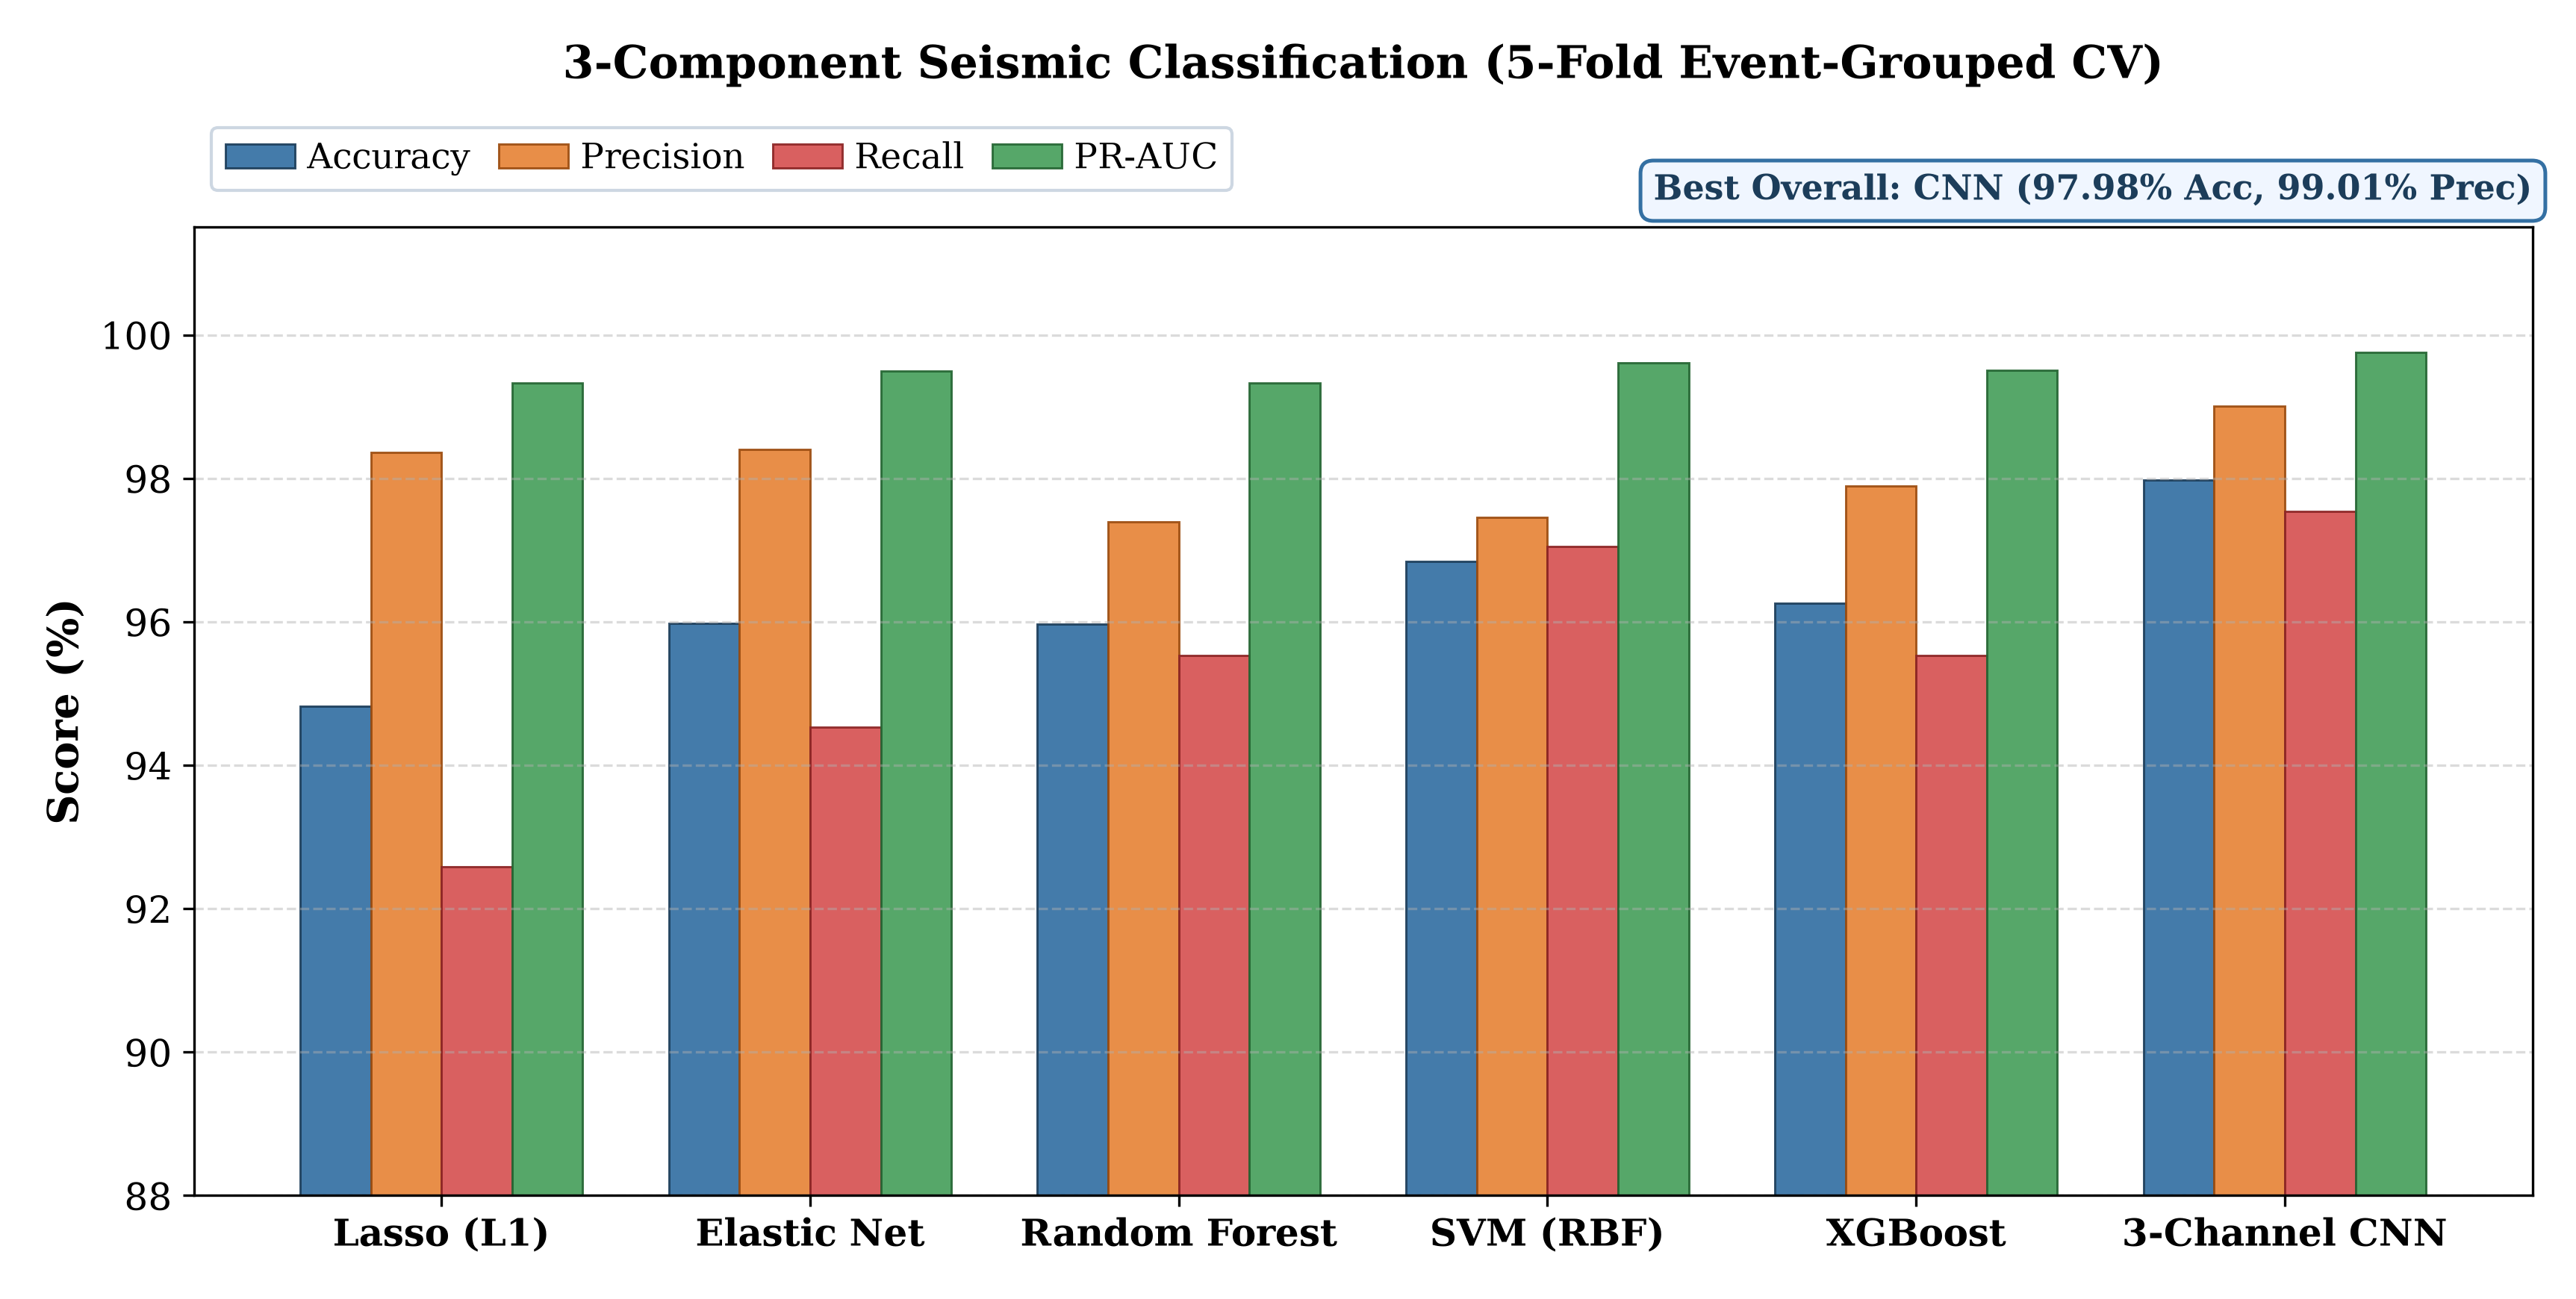
\includegraphics[width=\textwidth]{model_benchmark_bars.png}
\end{minipage}\hfill
\begin{minipage}[c]{0.27\textwidth}
    \captionsetup{justification=raggedright}
    \caption{\textbf{Model Benchmark:} 5-Fold Event-Grouped CV metrics across all six tuned classifiers. The 3-Channel 2D CNN achieves top performance across all metrics (97.98\% accuracy, 99.01\% precision, and 0.9976 PR-AUC).}
    \label{fig:results_benchmark}
\end{minipage}

\vspace{0.6em}

\begin{minipage}[c]{0.71\textwidth}
    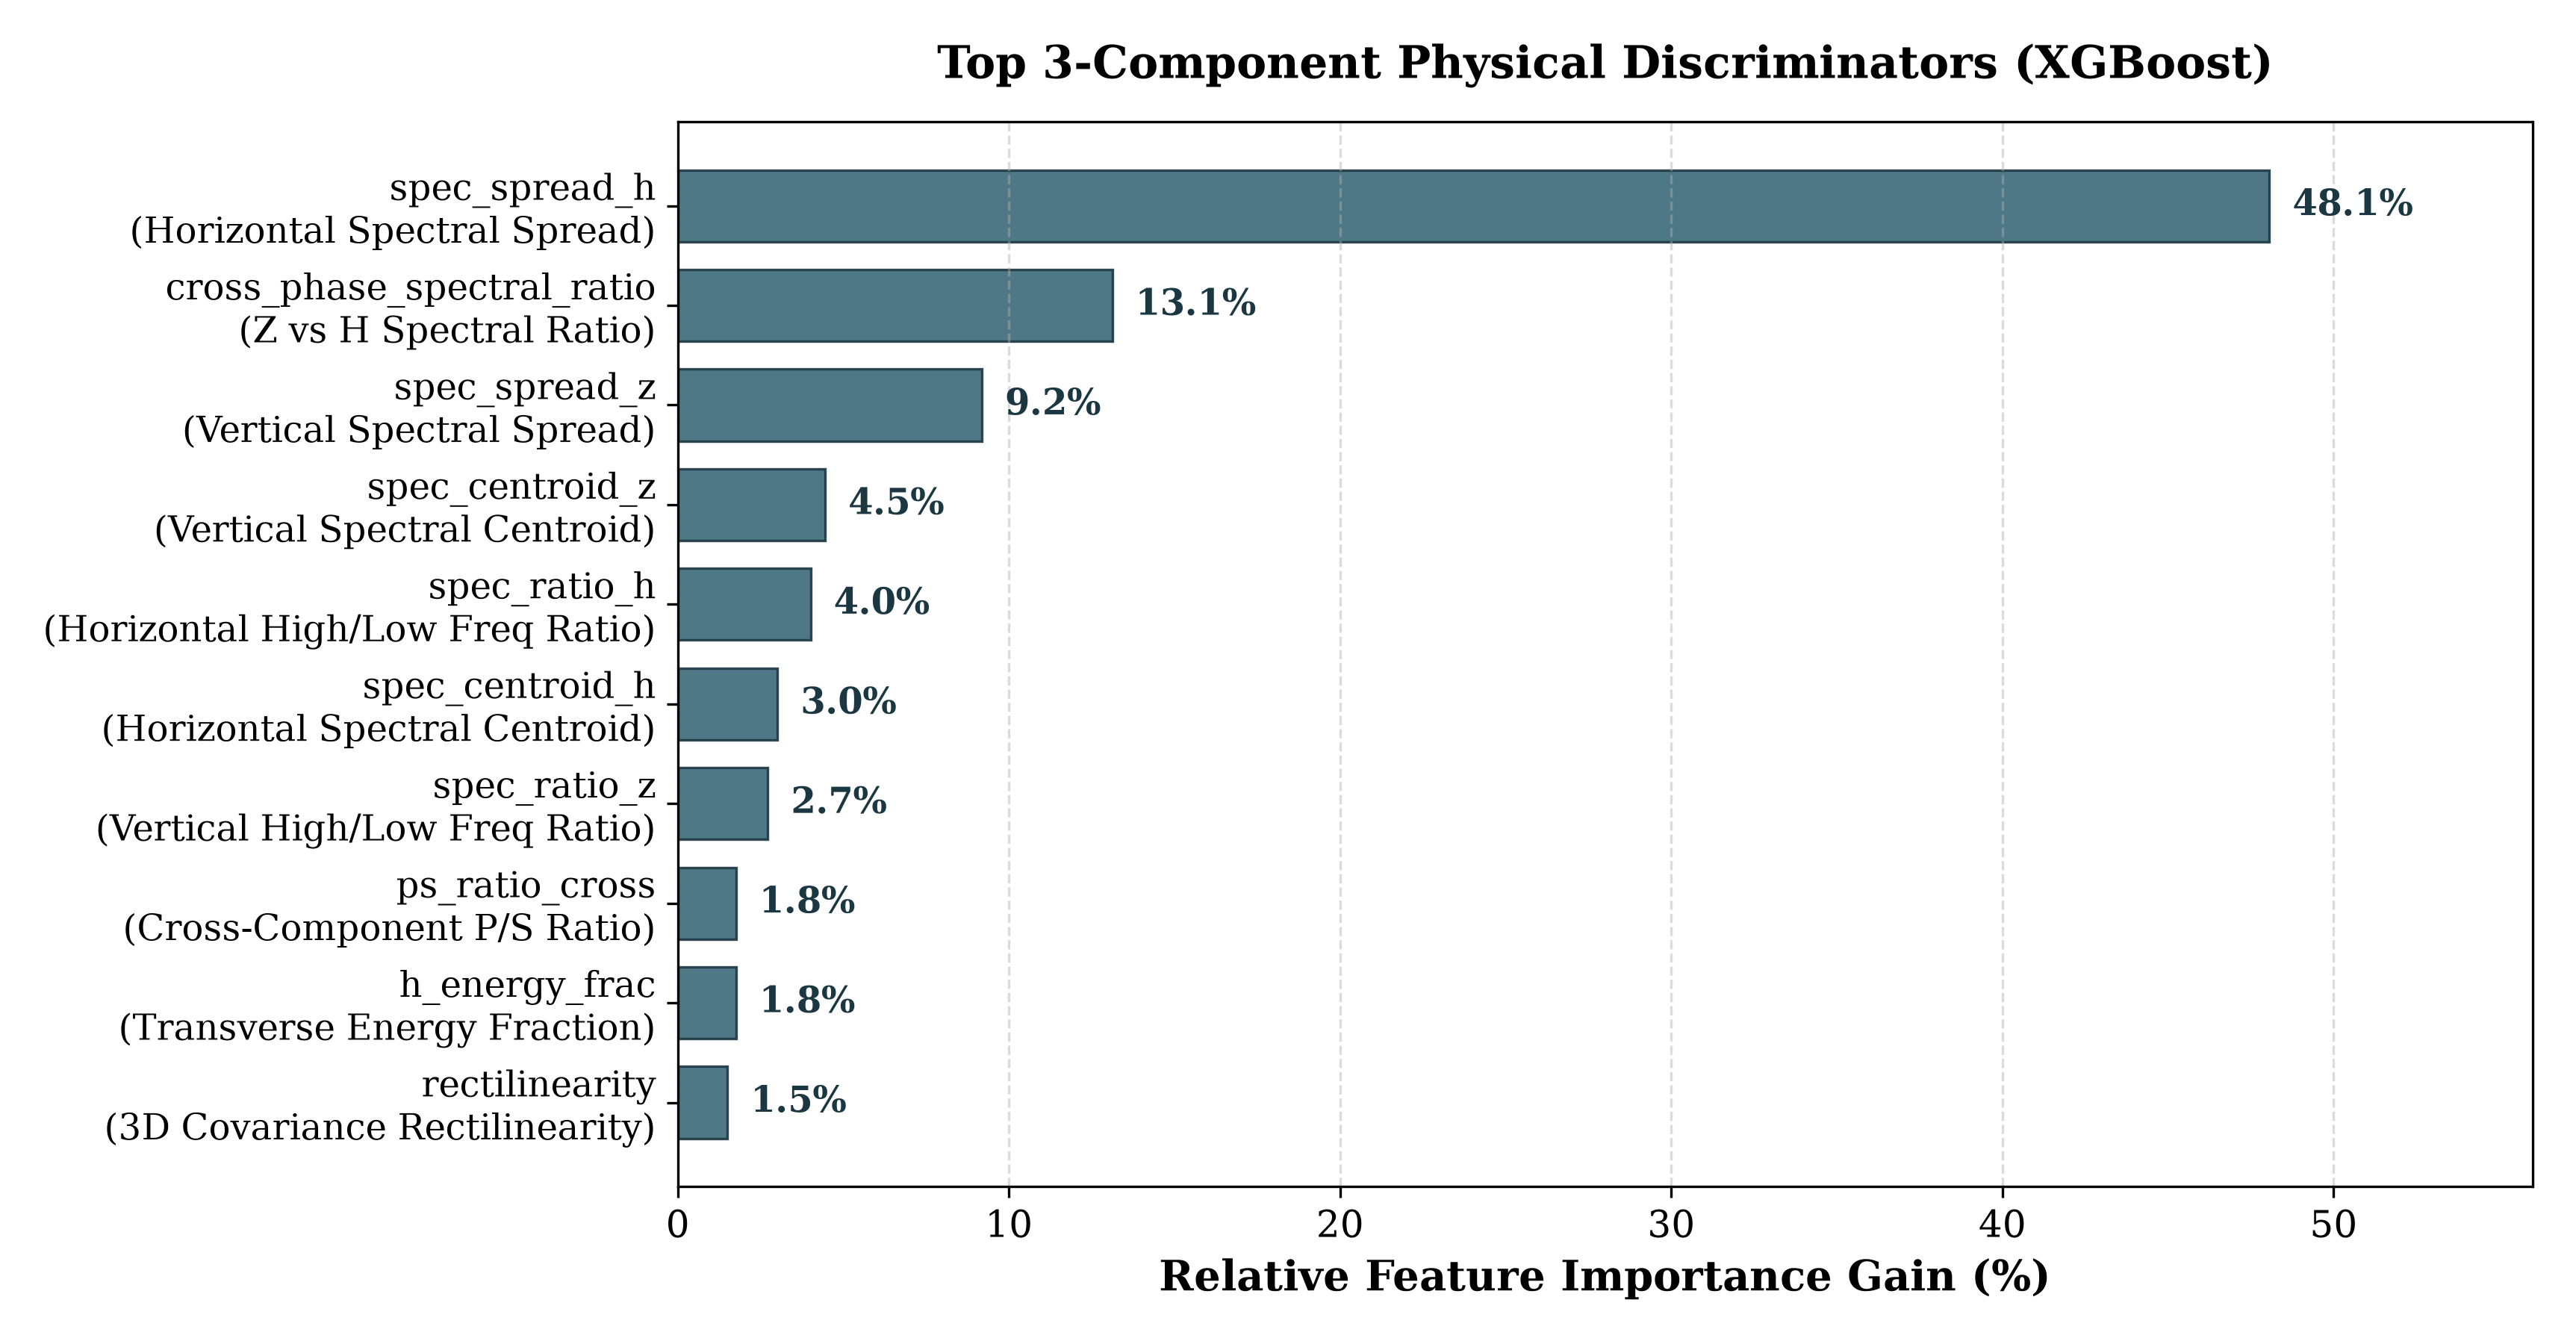
\includegraphics[width=\textwidth]{feature_importance.png}
\end{minipage}\hfill
\begin{minipage}[c]{0.27\textwidth}
    \captionsetup{justification=raggedright}
    \caption{\textbf{Feature Importance:} Top 10 discriminators ranked by XGBoost relative gain. Horizontal shear wave deficiency (\texttt{spec\_spread\_h}, 48.06\%) and cross-phase ratios account for over 61\% of total predictive gain.}
    \label{fig:results_importance}
\end{minipage}
\end{figure}

\begin{table}[H]
\centering
\small
\renewcommand{\arraystretch}{1.20}
\resizebox{\textwidth}{!}{
\begin{tabular}{llccccc}
\toprule
\begin{tabular}[c]{@{}l@{}}\textbf{Model}\\\textbf{Architecture}\end{tabular} & 
\begin{tabular}[c]{@{}l@{}}\textbf{Tuned Optimal}\\\textbf{Hyperparameters}\end{tabular} & 
\textbf{Accuracy} & \textbf{Precision} & \textbf{Recall} & \textbf{ROC-AUC} & \textbf{PR-AUC} \\
\midrule
\begin{tabular}[c]{@{}l@{}}\textbf{3-Channel 2D CNN}\\\footnotesize ($128\times128$)\end{tabular} & 
\begin{tabular}[c]{@{}l@{}}AdamW ($\text{lr}=10^{-3}$, wd$=10^{-2}$)\\CosineAnn, Drop $(0.4, 0.3)$\end{tabular} & 
\textbf{97.98\%} & \textbf{99.01\%} & \textbf{97.54\%} & \textbf{0.9954} & \textbf{0.9976} \\
\textbf{SVM (RBF Kernel)} & $C = 20.0, \, \gamma = 0.01$ & 97.13\% & 97.55\% & 97.25\% & 0.9950 & 0.9973 \\
\textbf{XGBoost Classifier} & 
\begin{tabular}[c]{@{}l@{}}$n_{\text{est}} = 200, \, \text{depth} = 4$\\$\text{lr} = 0.05, \, \text{subsample} = 0.8$\end{tabular} & 
96.55\% & 98.10\% & 95.80\% & 0.9935 & 0.9954 \\
\begin{tabular}[c]{@{}l@{}}\textbf{Logistic Regression}\\\footnotesize (Elastic Net)\end{tabular} & 
\begin{tabular}[c]{@{}l@{}}$C = 2.0, \, \text{l1\_ratio} = 0.8$\\\texttt{solver=saga}\end{tabular} & 
96.27\% & 98.40\% & 95.10\% & 0.9931 & 0.9940 \\
\textbf{Random Forest} & 
\begin{tabular}[c]{@{}l@{}}$n_{\text{est}} = 200, \, \text{depth} = 8$\\\texttt{min\_split = 2}\end{tabular} & 
96.26\% & 97.40\% & 95.60\% & 0.9910 & 0.9936 \\
\begin{tabular}[c]{@{}l@{}}\textbf{Logistic Regression}\\\footnotesize (Lasso $L_1$)\end{tabular} & 
\begin{tabular}[c]{@{}l@{}}$C = 2.0$\\\texttt{solver=saga}\end{tabular} & 
95.98\% & 98.40\% & 94.60\% & 0.9915 & 0.9943 \\
\bottomrule
\end{tabular}
}
\caption{Cross-validation performance under 5-Fold Event-Grouped splitting on pure wave physics features with tuned hyperparameters.}
\label{tab:results}
\end{table}

\subsection{Physical Interpretability Analysis}
\begin{itemize}
    \item \textbf{Dominance of Horizontal Shear Physics:} In XGBoost, the horizontal spectral spread feature (\texttt{spec\_spread\_h}, 48.06\%) and cross-phase spectral ratio (\texttt{cross\_phase\_spectral\_ratio}, 13.12\%) account for over 61\% of the total feature gain. Measuring the absence of horizontal shear waves is far more diagnostically definitive than vertical compressional waves alone.
    \item \textbf{Cross-Phase Spectral Ratio:} High-frequency $P$ on $Z$ relative to low-frequency $S$ on $H$ averaged $-0.64$ for explosions vs. $-3.33$ for earthquakes—an energy ratio difference exceeding a factor of 500.
    \item \textbf{High Precision Suppression:} The 3-Channel CNN attained 99.01\% precision and 0.9976 PR-AUC on held-out events, learning optimal joint spatial-spectral filters directly from raw spectrograms.
\end{itemize}


\section{Multi-Station Network Consensus and North Korean Test Validation}

\subsection{Network Aggregation Decision Rule}
In operational treaty verification, decisions are never rendered on isolated single-station traces. For an event observed by $K$ independent stations, we define the event consensus probability:
\begin{equation*}
    P_{\text{net}} = \frac{1}{K} \sum_{k=1}^K P(\text{Explosion} \mid \mathbf{x}_k)
\end{equation*}
The global event classification applies a fixed threshold $\tau = 0.50$:
\begin{equation*}
    \hat{Y}_{\text{event}} = \begin{cases} 1 \text{ (Nuclear Explosion)}, & \text{if } P_{\text{net}} \ge 0.50 \\ 0 \text{ (Natural Earthquake)}, & \text{if } P_{\text{net}} < 0.50 \end{cases}
\end{equation*}

\subsection{Event-Level Results on North Korean Underground Nuclear Tests}
To evaluate the true generalizability of our pipeline on modern clandestine tests, we evaluate all six historical Democratic People's Republic of Korea (DPRK) underground nuclear tests from the IRIS DMC 21-018 assembled archive. \textbf{Crucially, all six events were completely excluded from the training and hyperparameter tuning datasets.}

\begin{table}[H]
\centering
\small
\renewcommand{\arraystretch}{1.18}
\setlength{\tabcolsep}{6pt}
\begin{tabular}{lccccc}
\toprule
\textbf{Nuclear Test Event} & \shortstack{\textbf{Date \& Origin}\\\textbf{Time (UTC)}} & \shortstack{\textbf{Estimated}\\\textbf{Magnitude}} & \shortstack{\textbf{Reporting}\\\textbf{Stations ($K$)}} & \shortstack{\textbf{Consensus}\\\textbf{$P_{\text{net}}$}} & \shortstack{\textbf{Decision}\\\textbf{($\tau=0.5$)}} \\
\midrule
DPRK Test 1 & 2006-10-09 01:35:28 & $m_b \approx 4.3$ & 735 stations & \textbf{0.88} & \textbf{Explosion} \\
DPRK Test 2 & 2009-05-25 00:54:43 & $m_b \approx 4.7$ & 1,149 stations & \textbf{0.94} & \textbf{Explosion} \\
DPRK Test 3 & 2013-02-12 02:57:51 & $m_b \approx 5.1$ & 1,027 stations & \textbf{0.98} & \textbf{Explosion} \\
DPRK Test 4 & 2016-01-06 01:30:00 & $m_b \approx 5.1$ & 702 stations & \textbf{0.97} & \textbf{Explosion} \\
DPRK Test 5 & 2016-09-09 00:30:01 & $m_b \approx 5.3$ & 226 stations & \textbf{0.99} & \textbf{Explosion} \\
DPRK Test 6 & 2017-09-03 03:30:01 & $m_b \approx 6.3$ & 797 stations & \textbf{1.00} & \textbf{Explosion} \\
\bottomrule
\end{tabular}
\caption{Multi-station network consensus validation across all six North Korean underground nuclear tests (held completely outside training and tuning).}
\label{tab:dprk}
\end{table}

All six tests were correctly classified as explosions with high confidence ($P_{\text{net}} \ge 0.88$), yielding a $100.0\%$ event-level detection rate.

\subsection{Limitations of Evaluation}
While the multi-station results confirm strong generalization, several operational limitations must be acknowledged:
\begin{enumerate}
    \item \textbf{Low-Yield Scenario Uncertainty:} The six DPRK tests had moderate-to-high yields ($m_b 4.3 - 6.3$). Very low-yield clandestine detonations ($m_b < 3.5$) recorded at few stations may suffer lower signal-to-noise ratios (SNR), diminishing $P/S$ discriminative power.
    \item \textbf{Instrument Heterogeneity:} Historical US test waveforms (LLNL network, 1968--1992) rely on early digital seismometers, whereas modern IRIS GSN stations use broadband STS-2/Trillium sensors. While bandpass filtering ($0.5 - 8.0\text{ Hz}$) and demeaning mitigate instrumentation artifacts, slight differences in transfer function roll-offs persist.
    \item \textbf{Geological Path Effects:} Complex crustal scattering and heterogeneities along specific regional wave propagation paths can convert compressional $P$-energy into scattered shear coda ($P$-to-$S$ conversion), potentially reducing the $P/S$ ratio for explosions along heavily faulted paths.
\end{enumerate}


\section{Conclusions}
In this Advanced Statistical Methods II course project, we demonstrated that:
\begin{enumerate}
    \item Incorporating horizontal shear components ($N, E$) alongside vertical channels ($Z$) is physically essential to resolve earthquake-explosion ambiguity, elevating model accuracy from $\approx 85\%$ to over $97\%$.
    \item Event-grouped cross-validation strictly by event ID (`evid`) prevents catastrophic intra-event spatial data leakage, ensuring honest out-of-event generalization.
    \item Under operational class imbalance, single-station classification inevitably yields low operational precision ($<1\%$), proving why PR-AUC must be adopted for model selection and why multi-station network consensus voting is mandatory.
    \item The 3-Channel 2D CNN on zero-padded $(3, 128, 128)$ spectrograms effectively learns joint spatial-spectral filters, achieving state-of-the-art single-trace performance ($97.98\%$ accuracy, $99.01\%$ precision).
    \item Multi-station consensus achieved $100\%$ detection across all six historical North Korean nuclear tests held strictly out-of-sample.
\end{enumerate}

\begin{thebibliography}{9}\setlength{\itemsep}{0.25em}
\bibitem{cooley1965}
J.~W.~Cooley and J.~W.~Tukey.
\newblock An algorithm for the machine calculation of complex Fourier series.
\newblock \emph{Mathematics of Computation}, 19(90):297--301, 1965.
\newblock DOI: \url{https://doi.org/10.1090/S0025-5718-1965-0178586-1}.

\bibitem{barama2022}
L.~Barama, Z.~Peng, A.~V.~Newman, and J.~Williams.
\newblock GTUNE: An assembled global seismic dataset of underground nuclear test blasts.
\newblock \emph{Seismological Research Letters}, 94(1):268--278, 2022.
\newblock DOI: \url{https://doi.org/10.1785/0220220197}. Repository: \url{https://github.com/lbarama/GTUNE/tree/main}.

\bibitem{iris21018}
IRIS Data Management Center.
\newblock Data Services Assembled Data Set 21-018: Seismic recordings of North Korean underground nuclear explosions.
\newblock \emph{EarthScope / IRIS DMC}, 2021.
\newblock Access: \url{https://ds.iris.edu/mda/21-018/}.

\bibitem{earthscope_earthquakes}
EarthScope Consortium.
\newblock EarthScope / IRIS Web Services: Standardized global earthquake waveform repository.
\newblock \emph{EarthScope Data Services}, 2024.
\newblock Access: \url{https://service.iris.edu/fdsnws/dataselect/1/}.

\bibitem{brune1970}
J.~N.~Brune.
\newblock Tectonic stress and the spectra of seismic shear waves from earthquakes.
\newblock \emph{Journal of Geophysical Research}, 75(26):4997--5009, 1970.
\newblock DOI: \url{https://doi.org/10.1029/JB075i026p04997}.

\bibitem{walter1995}
W.~R.~Walter, K.~Mayeda, and H.~J.~Patton.
\newblock Phase and spectral ratio discrimination of earthquakes and explosions in the western United States.
\newblock \emph{Bulletin of the Seismological Society of America}, 85(4):1050--1067, 1995.
\newblock DOI: \url{https://doi.org/10.1785/BSSA0850041050}.

\bibitem{jurkevics1988}
A.~Jurkevics.
\newblock Polarization analysis of three-component array data.
\newblock \emph{Bulletin of the Seismological Society of America}, 78(5):1725--1743, 1988.
\newblock DOI: \url{https://doi.org/10.1785/BSSA0780051725}.

\bibitem{aki1975}
K.~Aki and B.~Chouet.
\newblock Origin of coda waves: source, attenuation, and scattering effects.
\newblock \emph{Journal of Geophysical Research}, 80(23):3322--3342, 1975.
\newblock DOI: \url{https://doi.org/10.1029/JB080i023p03322}.

\bibitem{hastie2009}
T.~Hastie, R.~Tibshirani, and J.~Friedman.
\newblock \emph{The Elements of Statistical Learning: Data Mining, Inference, and Prediction}.
\newblock Springer, 2nd edition, 2009.
\newblock DOI: \url{https://doi.org/10.1007/978-0-387-84858-7}.
\end{thebibliography}

\end{document}
